\begin{figure}[tbhp]
\centering
\includegraphics[width=\textwidth]{Figures/CD/BLOCK}
\caption{Block scheme of proposed methodology.}
\label{fig:1_method}
\end{figure}

% % % % Removing the headers
% \section{Proposed DNN based Framework}
\label{sec:Method}
In disaster relief and urban monitoring, typically CD analysis is applied in order to highlight the changed urban areas. On the other hand, a further analysis discriminating the unchanged urban areas from natural ones is desirable. Additionally, multi-temporal ground campaigns are often difficult and very few ground truth points may be available.   
%For disaster relief and urban monitoring operations, it is desirable to obtain simultaneous change and land-cover maps using very few training samples. 
The motivation behind this study is to develop a framework that can simultaneously perform accurate urban change detection and land-cover classification in a weakly supervised manner. The framework takes multi-temporal polarimetric SAR images as input and produces an output with 3 classes: changed urban areas, unchanged urban and unchanged natural areas. This kind of maps are useful for urban monitoring and rescue operations. %The two unchanged classes are also grouped to produce a binary urban change map. 

The  block scheme of the proposed methodology is shown in Figure~\ref{fig:1_method}. Two PolSAR images  acquired over the same geographic area at time instants $t_0$ and $t_1$,  are pre-processed and normalized  (Section~\ref{sub:pre})  before being given as input to a Stacked Auto-Encoder (AE) network (Section~\ref{sub:ae}). The AE is trained in an unsupervised manner to create an optimal representation, assuming that only a very small amount of ground truth is available, a label aggregation step is undertaken before classification by a Multi-layer Perceptorn (MLP) (Section~\ref{sub:weak}). 
The use of a AE with stacked features has the advantage of preserving both change and multi-temporal polarimetric scattering information which is exploited by the final classifier. % % DELETEABLE

%Muller matrices are derived from the data collected at time $t_0$ and $t_1$ .... parcel.... normalized in the range $[0,1]$ such that the histogram of the original data is preserved. This is simultaneously applied to the input of an stacked de-noised AE. The AE learns a representation that is able to maximally separate the changed areas from the unchanged areas. Since this representation also contains polarimetric information from both the Mueller matrices, in addition to identification of changed ares, it also is possible to classify the unchanged land-cover. 

%motivation
\begin{figure}[tbhp]
\centering
\includegraphics[width=0.6\columnwidth]{Figures/CD/SAE}
\caption{Block diagram of the unsupervised Stacked AE stage.}
\label{fig:SAE}
\end{figure}

\subsection{Data Preprocessing}
\label{sub:pre}
The full PolSAR complex backscattering matrix $\mathbf{S}$ consists of four independent measurements (HH, HV, VH and VV) with the phase relations preserved and is expressed as,
\begin{equation}
\mathbf{[S]} =
  \begin{bmatrix}
    S_{hh} & S_{hv}  \\
    S_{vh} & S_{vv}
  \end{bmatrix}
 \label{eqn:scattring}
\end{equation}
This can be expressed as Mueller matrix $\mathbf{M}$ as follows, 
\begin{equation}
\mathbf{M} = \mathbf{A}^* \left( \mathbf{S} \otimes \mathbf{S^{*}} \right) \mathbf{A^{-1}} 
\end{equation}
where,
\begin{equation} \small
\mathbf{A} = \begin{bmatrix}
    1 & 0 &  0 & 1 \\
    1 & 0 & 0&  -1\\ 
    0 & 1 &  1  &  0 \\
    0 & j  & -j & 0 \\
\end{bmatrix}
\end{equation}
Although when expressed in the backscatter convention, the matrix is named Kennaugh $\mathbf{K}$, it is common practice in literature to refer to it uniformly as $\mathbf{M}$. 

The $\mathbf{M}$ representation is constructed for images at $t_0$ and $t_1$.
Since SAR images are affected by speckle~\cite{lee1994speckle}, it is desirable to perform a smoothing or suppression step to reduce false alarms. A super-pixel (SP) based filtering technique is used. Simple Linear Iterative Clustering (SLIC) algorithm~\cite{6205760} with a perturbation window $n_w$ is applied on the Pauli composite of image acquired at $t_0$ to form super-pixels (SPs).  $\mathbf{M}$ is  averaged over SPs for both the $t_0$ and $t_1$ images to reduce the effect of speckle on the  change detection performance, This approach yields high edge preservation while providing maximum smoothing over homogeneous areas. 
The dynamic range of the dataset is  jointly normalized in the range $[0,1]$ for faster convergence of the optimization solver algorithm and  for efficient training of the network. 
%The Simple Linear Iterative Clustering (SLIC) algorithm~\cite{6205760} with a perturbation window $n_w$ is applied on the Pauli composite of image at $t_0$ to form super-pixels (SPs). The $\mathbf{M}$ is then averaged over these SPs for both the $t_0$ and $t_1$ images to reduce the effect of speckle on the final change detection performance. This approach yields high edge preservation while providing maximum smoothing over homogeneous areas. This characteristic is desirable for training the AE. 
  %SLIC
 
%\subsection{Superpixel}
%Since SAR images are affected by speckle~\cite{lee1994speckle}, it is desirable to perform a smoothing or suppression step to reduce false alarms. An adaptive window based  based on the SLIC algorithm~\cite{6205760} with a perturbation window $n_w$ is applied on the Pauli composite of image at $t_0$. The $\mathbf{M}$ is then averaged over this windows  for both the $t_0$ and $t_1$ images. 

%\subsection{Normalization}
%The $\mathbf{M}$ representation is real valued allowing 


% SLIC? 
%\subsubsection{Unsupervised Representation Learning using a Stacked Auto-Encoder Network}
\subsection{Unsupervised Representation Learning using Auto-Encoders}
\label{sub:ae}

The pre-processed $\mathbf{M}$ elements from the image pair for each corresponding pixel is stacked together  to form the input vector $x$, which is given to stacked AE (Figure~\ref{fig:SAE}). The objective of the AE is to reconstruct output $x'$ to match $x$ as closely as possible. The loss function of the AE is modified to be a combination of L2 norm and Cross Entropy error given by,

\begin{dmath} 
E = \lambda_{w1} \frac{-1}{N}\sum_{n=1}^{N}[x_n \log \hat{x_n} + (1 - x_n)\log(1-\hat{x_n})] 
     + \lambda_{w2} \frac 1 {2N} \sum_{i=1}^N \| x^1_i - x^2_i \|_2^2
\end{dmath}

where $\lambda_{w1},\lambda_{w2},$ are the loss weighting parameters, $N$ is the total number of samples in the dataset and $E$ is the total loss evaluated for back-propagation. This modified loss function leads to a representation that maximally separates changed from unchanged areas. Further to prevent over fitting, a weight decay strategy is applied with the regularization term $\lambda \sum_{i=0}^{|N|} (x_i-x'_i)^2$, where $\lambda$ is the decay parameter. Since $|N|$ is quite large for the complete dataset, the optimization is performed in smaller mini-batches of $D << |N|$. Regularization constrains the AE to be less sensitive to the input, but in minimization of the reconstruction error, it remains sensitive to variations along the manifold of high density. %~\cite{bengio2013representation}.  

%\subsection{PCA}
After  training, the representational layer $z$ is extracted as a feature from the AE. Principle Component Analysis (PCA) is applied to transform $z$  to a set of linearly uncorrelated variables $PC_1, PC_2... PC_n$ by projection into the eigenvector space. The information content in each $PC$ is evaluated by ordering the set of eigenvalues and considering the corresponding top $k$ $PCs$ for label aggregation. 

\begin{figure}[tbhp]
\centering
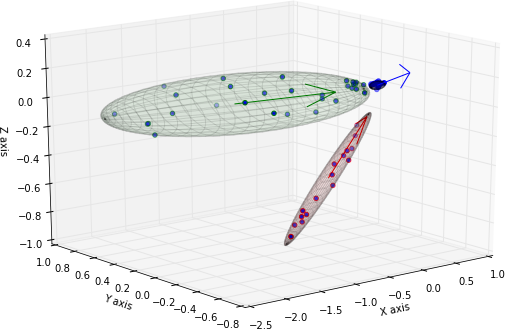
\includegraphics[width=0.8\columnwidth]{Figures/CD/3d}
\caption{Mechanism of MVBE fitting for labeled sample generation in the PC space.}
\label{fig:MVE}
\end{figure}

%\subsubsection{Weakly Supervised Classification using Feed Forward Network}
\subsection{Weakly Supervised Classification}
\label{sub:weak}
Ground reference labels are assumed to be available for only a small portion of the scene. This is a realistic assumption for disaster relief or monitoring efforts, where information would be available at a point of the scene where administrative efforts are concentrated. However the total number of labeled pixels  is $l << N$ and hence the framework is said to be weakly supervised. The use of very few samples  will lead to poor accuracies as the dataset is under-represented. Thus a label aggregation step is performed. In the $PC_k$ space a convex-hull is fitted for each class on the labeled samples, in order to reduce the number of considered points and simplify computation. Then a minimum volume bounding ellipsoid (MVBE) is fitted on these points as illustrated in Figure~\ref{fig:MVE}. Thinning along the radial axis of the ellipsoid is performed to exclude points that lie on the periphery of the volume, having a lower probability of belonging to the class than a more internal point. After thinning, points that lie within each ellipsoid are assumed to belong to the corresponding class and are preselected for labeling. From these, an equal number of samples $L$ are chosen per-class using the reservoir sampling technique to preserve the distribution of each class. These  samples are then to assigned the corresponding class labels, increasing the number of labeled samples available to the final classifier.  
% % EQUATIONs And figures
A Multi-Layer Perceptron (MLP) network is used to perform the final classification with the aggregated labels. The extracted representation $z$ is used in the classification with the aggregated labels to produce the final output map. %This represents both the changed urban areas and a land-cover classification of the unchanged areas: simultaneously generating an urban change and extent map.








